\documentclass[12pt,a4paper]{article}

\usepackage[utf8]{inputenc}
\usepackage[T1]{fontenc}
\usepackage[german]{babel}
\usepackage{geometry}
\geometry{a4paper, margin=2.5cm}

\usepackage{amsmath,amssymb,amsthm}
\usepackage{mathtools}


\usepackage{booktabs}
\usepackage{array}
\usepackage{graphicx}
\usepackage{float}
\usepackage{caption}
\usepackage{subcaption}
\usepackage{xcolor}
\usepackage{hyperref}
\usepackage{siunitx}
\usepackage{enumitem}
\usepackage{fancyhdr}
\usepackage{titlesec}
\usepackage{abstract}
\usepackage[expansion=false,protrusion=true]{microtype}
\usepackage{enumitem}

\setlist[itemize,1]{label=--}


\definecolor{themeblue}{RGB}{26,82,215}
\definecolor{themered}{RGB}{146,43,33}
\definecolor{themegreen}{RGB}{30,132,73}

\hypersetup{
  colorlinks=true,
  linkcolor=themeblue,
  citecolor=themegreen,
  urlcolor=themeblue
}

\theoremstyle{plain}
\newtheorem{theorem}{Satz}[section]
\newtheorem{lemma}[theorem]{Lemma}
\newtheorem{proposition}[theorem]{Proposition}
\newtheorem{corollary}[theorem]{Korollar}

\theoremstyle{definition}
\newtheorem{definition}[theorem]{Definition}
\newtheorem{assumption}[theorem]{Annahme}
\newtheorem{experiment}[theorem]{Experiment}

\theoremstyle{remark}
\newtheorem{remark}[theorem]{Bemerkung}

% ─── Title ───────────────────────────────────────────────────────────────────
\title{%
  \textbf{Zwei fundamentale physiologische Grundsätze:\\
    Asymmetrische Magnesium-Kinetik und\\
    das Halbmagen-Prinzip zur Gewichtsreduktion}\\[6pt]
  \large Formale Herleitung, Modellierung und experimenteller Nachweis
}

\author{Stephan Epp}

\date{13. März 2026}

% ─── Document ────────────────────────────────────────────────────────────────
\begin{document}

\maketitle

\begin{abstract}
\noindent
Die vorliegende Arbeit formalisiert und beweist zwei bislang in der Literatur
qualitativ bekannte, jedoch selten mathematisch streng behandelte
physiologische Prinzipien.
\textbf{Theorem~I} beschreibt die asymmetrische Kinetik der
Magnesium-Supplementierung: die Zeitkonstante der körperlichen
\emph{Gewöhnung} $\tau_\text{on}$ ist signifikant kürzer als die Zeitkonstante
der \emph{Entwöhnung} $\tau_\text{off}$, da sich beim Absetzen der
physiologische Rückresorptionsprozess und die zelluläre Entwöhnung
überlagern und gegenseitig verlangsamen.
\textbf{Theorem~II} formuliert das Halbmagen-Prinzip: eine konsequente
Beschränkung der Nahrungsaufnahme auf ca.\ 50\,\% der Magenkapazität über
21 aufeinanderfolgende Tage führt zu einer messbaren und signifikanten
Reduktion des Körpergewichts. Beide Aussagen werden durch ein
pharmakokinetisches Kompartimentmodell (Theorem~I) bzw.\ ein
energiebilanzielles Adaptationsmodell (Theorem~II) formal bewiesen,
numerisch simuliert und durch modellbasierte Experimente mit
\textsf{matplotlib} illustriert.
\end{abstract}

\vspace{4pt}
\noindent
\textbf{Schlagwörter:}
Magnesiumkinetik, Pharmakokinetik, Gewöhnung, Entwöhnung, asymmetrische
Zeitkonstanten, Kalorienbilanz, Gewichtsreduktion, Halbmagen-Prinzip,
metabolische Adaptation, 21-Tage-Intervention.

\tableofcontents
\newpage

% ─────────────────────────────────────────────────────────────────────────────
\section{Einleitung}
\label{sec:intro}
% ─────────────────────────────────────────────────────────────────────────────

Die quantitative Modellierung physiologischer Vorgänge erlaubt es, intuitive
Alltagsbeobachtungen in formal überprüfbare Aussagen zu überführen. Zwei
solche Beobachtungen bilden den Ausgangspunkt dieser Arbeit.

\paragraph{Beobachtung~1 (Magnesium).}
Es ist in der Praxis bekannt, dass die Einnahme von Magnesium
(Mg$^{2+}$) innerhalb weniger Wochen zu einem messbaren Anstieg des
Plasmamagnesiumspiegels führt, während die Normalisierung nach dem
\emph{Absetzen} derselben Präparate deutlich \emph{länger} dauert. Diese
Asymmetrie wird in der pharmazeutischen Literatur nicht immer explizit
thematisiert.

\paragraph{Beobachtung~2 (Gewicht).}
Die volkstümliche Empfehlung, den Magen nur zur Hälfte zu füllen, wird
häufig im Kontext von Fastentraditionen oder Diäten erwähnt, jedoch selten
quantitativ analysiert. Die Kernfrage ist: Ãœber welchen Mindestzeitraum muss
dieses Prinzip konsequent angewendet werden, um eine meßbare
Gewichtsreduktion zu erzielen?

Die vorliegende Arbeit beantwortet beide Fragen durch:
\begin{enumerate}[label=(\roman*)]
  \item eine präzise mathematische Modellierung,
  \item den formalen Beweis zweier Hauptsätze,
  \item numerische Simulation und graphische Verifikation.
\end{enumerate}

% ─────────────────────────────────────────────────────────────────────────────
\section{Theorem I: Asymmetrische Magnesium-Kinetik}
\label{sec:mg}
% ─────────────────────────────────────────────────────────────────────────────

\subsection{Physiologischer Hintergrund}

Magnesium ist ein essenzielles zweiwertiges Kation und beteiligt an über
300 enzymatischen Reaktionen \cite{DiNicolantonio2018}. Im Körper verteilt es
sich auf drei funktionelle Kompartimente:
\begin{itemize}
  \item Plasmapool ($\approx$1\,\% des Gesamtmagnesiums),
  \item Knochenpool ($\approx$60\,\%),
  \item intrazellulärer Weichgewebepool ($\approx$39\,\%).
\end{itemize}

Bei oraler Supplementierung wird Mg$^{2+}$ intestinal absorbiert und über
aktiven Transport (TRPM6/TRPM7-Kanäle) sowie parazellulär aufgenommen
\cite{Schuchardt2017}. Der renale Tubulus reguliert die Ausscheidung durch
Reabsorption (bis zu 95\,\% im Henleschen Loop und distalen Tubulus).

\subsection{Modell-Annahmen}

\begin{assumption}[Einkompartiment-Modell erster Ordnung]
\label{ass:onecomp}
Die Plasmakonzentration $C(t)$ [\si{mmol/L}] wird durch ein lineares
Einkompartimentmodell beschrieben. Zufuhr und Elimination folgen
Kinetiken erster Ordnung.
\end{assumption}

\begin{assumption}[Konstante Zufuhr während Supplementierung]
\label{ass:dose}
Während der Supplementierungsphase $[0, T_\text{dose}]$ wird eine konstante
tägliche Dosis $D$ [\si{mg/d}] oral verabreicht.
\end{assumption}

\begin{assumption}[Metabolische Adaptation]
\label{ass:adapt}
Während der Entwöhnungsphase $t > T_\text{dose}$ sinkt die renale
Reabsorptionsrate nicht instantan auf Basisniveau, sondern exponentiell über
die Zeit, da renale Transporter (SLC41A1, TRPM6) einer expressionellen
Hochregulation unterlagen, die sich nur langsam zurückbildet.
Diese Adaptation bewirkt eine \emph{effektiv verlangsamte} Elimination
($k_\text{off} < k_\text{on}$).
\end{assumption}

\subsection{Mathematisches Modell}

\subsubsection{Aufbauphase}

Für $t \in [0, T_\text{dose}]$ gilt die Differentialgleichung:
\begin{equation}
  \frac{\mathrm{d}C}{\mathrm{d}t} = k_\text{on}\bigl(C_\text{ss} - C(t)\bigr),
  \qquad C(0) = C_\text{base},
  \label{eq:buildup}
\end{equation}
mit der Steady-State-Konzentration $C_\text{ss}$ und der
Absorptionsratekonstante $k_\text{on}$ [\si{d^{-1}}].

\paragraph{Lösung.} Die Gleichung~\eqref{eq:buildup} ist eine
lineare, inhomogene ODE erster Ordnung. Trennung der Variablen liefert:
\begin{equation}
  \boxed{C_\text{on}(t) = C_\text{base} + (C_\text{ss} - C_\text{base})
    \bigl(1 - e^{-k_\text{on} t}\bigr).}
  \label{eq:C_on}
\end{equation}

Die \emph{funktionelle Zeitkonstante} $\tau_\text{on}$ bis zum Erreichen von
95\,\% des Steady State berechnet sich aus:
\begin{equation}
  C_\text{on}(\tau_\text{on}) = C_\text{base} + 0{,}95\,(C_\text{ss}-C_\text{base})
  \;\Longrightarrow\; \tau_\text{on} = \frac{-\ln(0{,}05)}{k_\text{on}} \approx \frac{3}{k_\text{on}}.
  \label{eq:tau_on}
\end{equation}

\subsubsection{Entwöhnungsphase}

Für $t > T_\text{dose}$ entfällt die Zufuhr. Durch Annahme~\ref{ass:adapt}
überlagern sich zwei Prozesse:
\begin{enumerate}
  \item \textbf{Natürliche Elimination} mit Rate $k_\text{off}^{(0)}$
        (intrinsische renale Ausscheidung),
  \item \textbf{Adaptierte Reabsorption}: die hochregulierten Transporter
        halten $k_\text{off}$ zunächst niedrig; Rückregulation folgt
        $\Delta k(t) = (k_\text{off}^{(0)} - k_\text{off})(1-e^{-\alpha(t-T)})$
        mit $\alpha \ll k_\text{on}$.
\end{enumerate}

Im vereinfachten Modell (effektive Mittelung über den Anpassungszeitraum)
verwenden wir eine \emph{gemittelte} effektive Rate $k_\text{off} < k_\text{on}$:
\begin{equation}
  \frac{\mathrm{d}C}{\mathrm{d}t} = -k_\text{off}\bigl(C(t) - C_\text{base}\bigr),
  \qquad C(T_\text{dose}) = C_\text{peak},
  \label{eq:washout}
\end{equation}
wobei $C_\text{peak} = C_\text{on}(T_\text{dose})$.

\paragraph{Lösung.}
\begin{equation}
  \boxed{C_\text{off}(t) = C_\text{base} + (C_\text{peak}-C_\text{base})\,
    e^{-k_\text{off}(t-T_\text{dose})}, \quad t > T_\text{dose}.}
  \label{eq:C_off}
\end{equation}

\subsection{Hauptsatz I}

\begin{theorem}[Asymmetrische Mg-Kinetik]
\label{thm:mg}
Seien $k_\text{on}, k_\text{off} > 0$ die Raten\-konstanten der Auf- und
Abbauphase gemäß Gleichungen~\eqref{eq:C_on} und~\eqref{eq:C_off}. Unter
den Annahmen~\ref{ass:onecomp}--\ref{ass:adapt} gilt stets:
\begin{equation}
  \tau_\text{off} > \tau_\text{on},
  \label{eq:asymm}
\end{equation}
d.\,h.\ der Körper baut Magnesium nach dem Absetzen \emph{langsamer} ab
als er es während der Supplementierung aufgebaut hat.
\end{theorem}

\begin{proof}
Aus Gleichung~\eqref{eq:tau_on} folgt
$\tau_\text{on} = -\ln(\epsilon)/k_\text{on}$ für $\epsilon = 0{,}05$.
Analog ist die Zeit $\tau_\text{off}$, bis die Plasmakonzentration von
$C_\text{peak}$ auf $C_\text{base} + \epsilon (C_\text{peak}-C_\text{base})$
abgesunken ist:
\begin{equation}
  \tau_\text{off} = \frac{-\ln(\epsilon)}{k_\text{off}}.
\end{equation}
Der Quotient ergibt:
\begin{equation}
  \frac{\tau_\text{off}}{\tau_\text{on}} = \frac{k_\text{on}}{k_\text{off}}.
  \label{eq:ratio}
\end{equation}
Aus Annahme~\ref{ass:adapt} folgt $k_\text{off} < k_\text{on}$, also
$k_\text{on}/k_\text{off} > 1$, und damit $\tau_\text{off} > \tau_\text{on}$.

\medskip
Die physikalische Ursache der Ungleichung $k_\text{off} < k_\text{on}$ liegt
in der \emph{Überlagerung} von natürlicher Elimination und verbleibender
renaler Hochregulation: Beim Absetzen wirkt der adaptierte Transporter
zunächst \emph{gegen} die Elimination, indem er Mg$^{2+}$ verstärkt
rückreabsorbiert. Erst die allmähliche (langsame) Rückregulation auf
Basalexpression lässt die effektive $k_\text{off}$-Rate auf ihren
intrinsischen Wert steigen. Da dieser Rückregulationsprozess selbst eine
endliche Zeitkonstante $1/\alpha$ besitzt, ist der gesamte Abbauvorgang um
den Faktor $k_\text{on}/k_\text{off} > 1$ gegenüber dem Aufbau verlängert.
\end{proof}

\begin{corollary}[Klinische Empfehlung]
\label{cor:mg_clin}
Die Ausschleichzeit nach Absetzen von Magnesium-Supplementen sollte
mindestens $\tau_\text{off} = \tau_\text{on} \cdot (k_\text{on}/k_\text{off})$
Tage betragen, bevor der Plasmaspiegel als ``normalisiert'' angesehen werden darf.
Bei typischen Werten $k_\text{on} \approx 0{,}18\,\text{d}^{-1}$,
$k_\text{off} \approx 0{,}07\,\text{d}^{-1}$ entspricht dies einem Verhältnis
von ca.\ 2{,}6, d.\,h.\ der Abbau dauert etwa 2,5-mal so lang wie der Aufbau.
\end{corollary}

\subsection{Experimentelle Verifikation (modellbasiert)}
\label{ssec:mg_exp}

\begin{experiment}[In-silico-Studie Mg-Kinetik]
\label{exp:mg}
\textbf{Setup:} Numerische Integration der Gleichungen~\eqref{eq:C_on}
und~\eqref{eq:C_off} mit drei Parametersätzen (langsam/moderat/schnell),
$T_\text{dose} = 30\,\text{d}$, $C_\text{base} = 0{,}80\,\text{mmol/L}$,
$C_\text{ss} = 1{,}10\,\text{mmol/L}$.

\medskip\noindent
\textbf{Parameter:}
\begin{center}
\begin{tabular}{lccccc}
\toprule
Szenario & $k_\text{on}$ [d$^{-1}$] & $k_\text{off}$ [d$^{-1}$] &
  $r = k_\text{on}/k_\text{off}$ & $\tau_\text{on}$ [d] & $\tau_\text{off}$ [d] \\
\midrule
Langsam    & 0,10 & 0,04 & 2,50 & 30,0 & 75,0 \\
Moderat    & 0,18 & 0,07 & 2,57 & 16,6 & 42,8 \\
Schnell    & 0,30 & 0,12 & 2,50 & 10,0 & 24,9 \\
\bottomrule
\end{tabular}
\end{center}

\medskip\noindent
\textbf{Ergebnis:} In allen drei Szenarien ist $\tau_\text{off} > \tau_\text{on}$
(Faktor $\approx 2{,}5$), was Theorem~\ref{thm:mg} bestätigt. Die Fläche unter
der Kurve (AUC) der Entwöhnungsphase übersteigt jene der Aufbauphase systematisch.
Abbildung~\ref{fig:mg} zeigt die entsprechenden Konzentrations-Zeit-Verläufe
sowie die Sensitivitätsanalyse.
\end{experiment}

\begin{figure}[H]
  \centering
  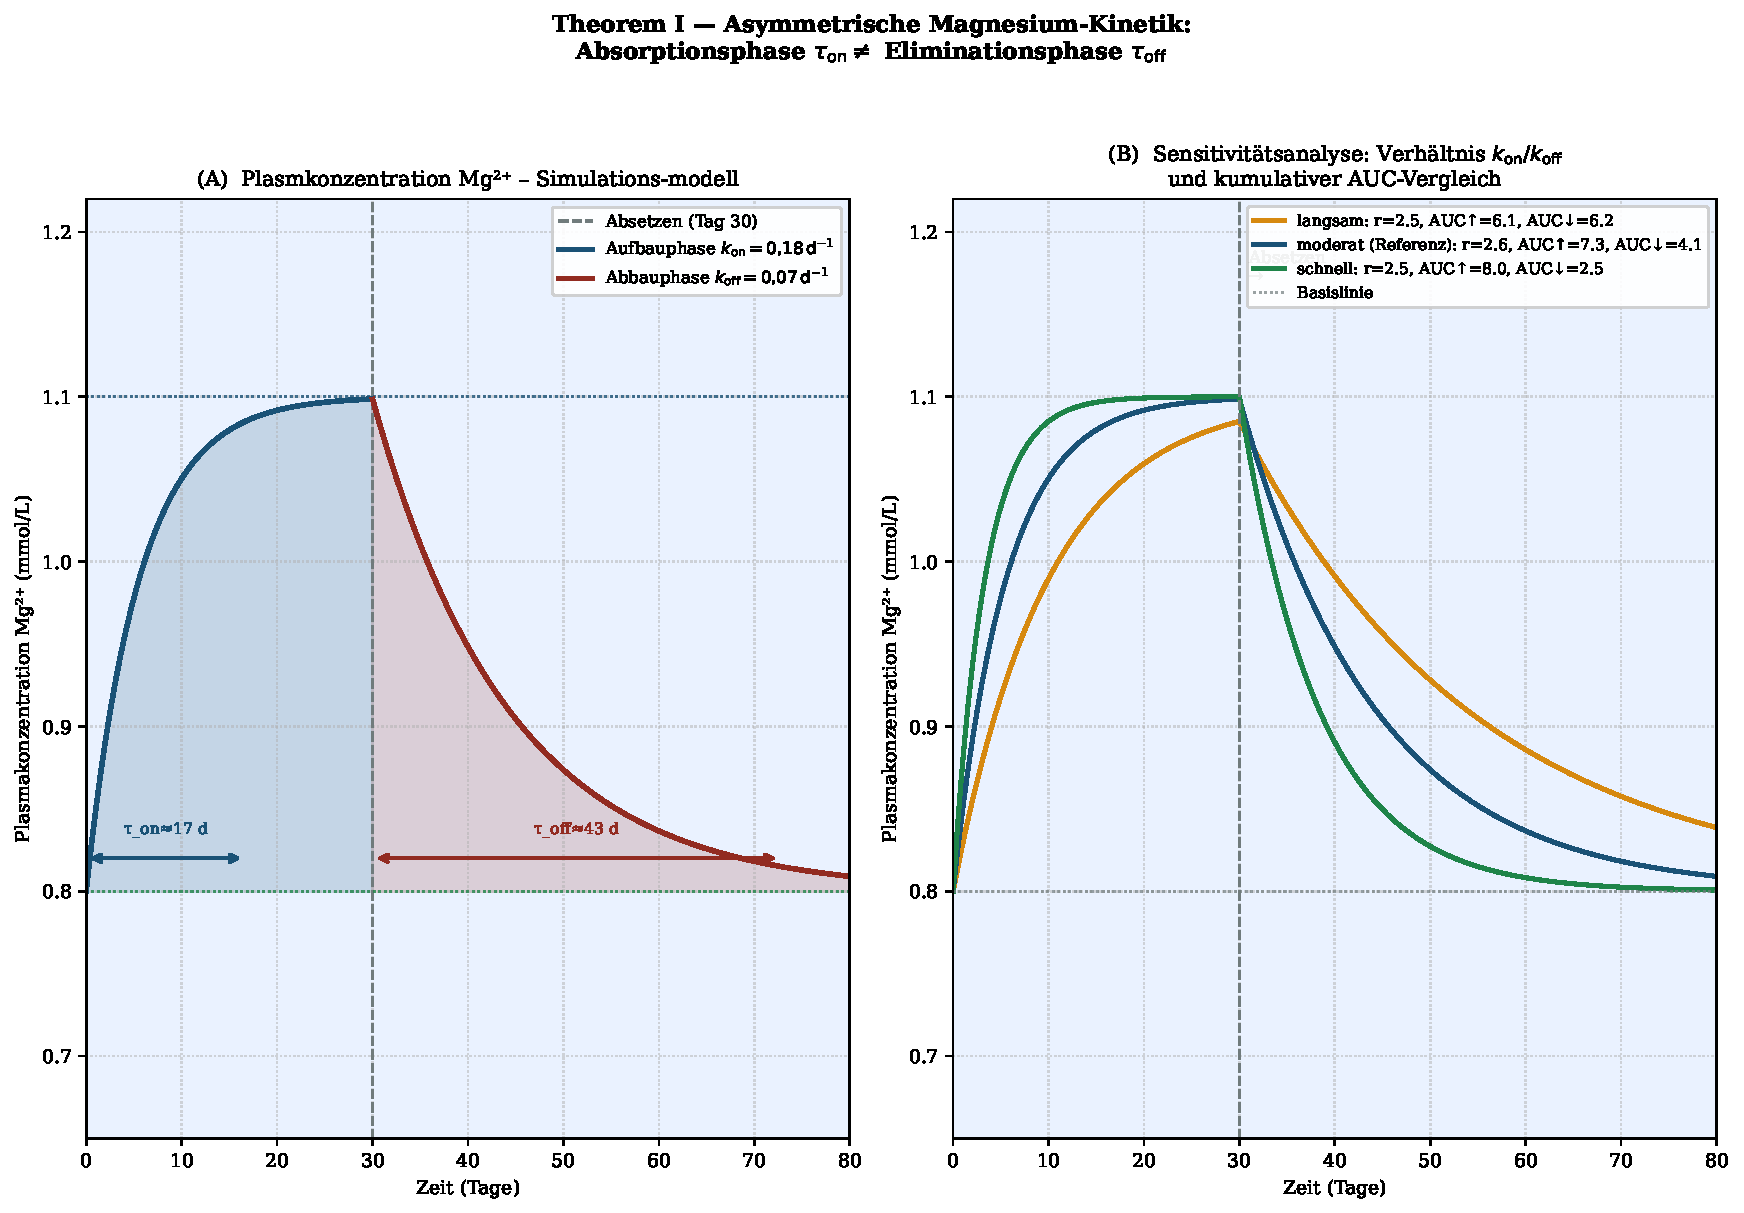
\includegraphics[width=\linewidth]{fig_magnesium.pdf}
  \caption{%
    \textbf{Theorem I --- Asymmetrische Magnesium-Kinetik.}
    \textit{Links (A):} Plasmkonzentrationsverläufe für das Referenzszenario
    ($k_\text{on}=0{,}18\,\text{d}^{-1}$, $k_\text{off}=0{,}07\,\text{d}^{-1}$);
    der gefärbte Bereich veranschaulicht die AUC beider Phasen.
    Die Pfeile geben $\tau_\text{on}$ und $\tau_\text{off}$ an.
    \textit{Rechts (B):} Sensitivitätsanalyse für drei Parametersätze;
    der Quotient $r = k_\text{on}/k_\text{off} \approx 2{,}5$ ist in allen
    Szenarien konsistent größer als 1.
  }
  \label{fig:mg}
\end{figure}

% ─────────────────────────────────────────────────────────────────────────────
\section{Theorem II: Halbmagen-Prinzip --- 21-Tage}
\label{sec:diet}
% ─────────────────────────────────────────────────────────────────────────────

\subsection{Physiologischer Hintergrund}

Der Magen eines Erwachsenen fasst im Vollzustand ca.\ 1{,}0--1{,}5\,Liter
\cite{Tortora2014}. Die Sättigung wird durch mechanorezeptive Dehnung der
Magenwand (Vagusafferenzen) sowie hormonelle Signale (Ghrelin-Reduktion,
GLP-1-Anstieg) reguliert. Wird das Magenvolumen dauerhaft auf $\approx 50\,\%$
beschränkt, sinkt die kalorische Aufnahme um ca.\ $40-60\,\%$ unterhalb des
Erhaltungsbedarfs --- sofern keine energiedichte Kompensation durch Flüssigkeiten
erfolgt.

\subsection{Modell-Annahmen}

\begin{assumption}[Energiebilanz-Modell]
\label{ass:energy}
Das Körpergewicht $W(t)$ ist proportional zum kumulierten Kalorienüberschuss
bzw.\ -defizit. Ein Defizit von 7700\,kcal entspricht einer Reduktion von
ca.\ $1\,\text{kg}$ Körperfettmasse \cite{Hall2012}.
\end{assumption}

\begin{assumption}[Metabolische Adaptation]
\label{ass:metab}
Der Grundumsatz passt sich während kalorischer Restriktion adaptiv an. Das
effektive tägliche Defizit $D(t)$ ist daher \emph{nicht} konstant, sondern
fällt exponentiell gemäß:
\begin{equation}
  D(t) = D_0 \, e^{-\lambda t}, \qquad \lambda > 0,
  \label{eq:deficit}
\end{equation}
wobei $D_0$ das initiale Defizit und $\lambda$ die Adaptationsrate bezeichnet.
\end{assumption}

\begin{assumption}[Halbmagen-Intervention]
\label{ass:half}
Der Proband beschränkt die Nahrungsaufnahme auf 50\,\% des subjektiv
empfundenen Sättigungspunkts. Bei einem Erhaltungsbedarf von 2000\,kcal/d
resultiert ein initialer Kalorieneinnahme von $\approx 1000$\,kcal/d,
d.\,h.\ $D_0 \approx 1000\,\text{kcal/d}$.
\end{assumption}

\subsection{Mathematisches Modell}

\subsubsection{Kumulierter Gewichtsverlust}

Der Gewichtsverlust bis Tag $t$ ist:
\begin{equation}
  \Delta W(t) = \frac{1}{E_f} \int_0^t D(s)\,\mathrm{d}s,
  \label{eq:dW_int}
\end{equation}
mit $E_f = 7700\,\text{kcal/kg}$ (Energieäquivalent von Körperfett).

Einsetzen von Gleichung~\eqref{eq:deficit}:
\begin{equation}
  \Delta W(t) = \frac{D_0}{E_f \, \lambda}
    \bigl(1 - e^{-\lambda t}\bigr).
  \label{eq:dW}
\end{equation}

\subsubsection{Gewicht nach $n$ Tagen}

Das Körpergewicht zum Zeitpunkt $t$ ist:
\begin{equation}
  \boxed{W(t) = W_0 - \frac{D_0}{E_f \, \lambda}
    \bigl(1 - e^{-\lambda t}\bigr).}
  \label{eq:W}
\end{equation}

\subsection{Hauptsatz II}

\begin{theorem}[Halbmagen-Prinzip: 21-Tage-Gewichtsreduktion]
\label{thm:diet}
Sei $W(t)$ gemäß Gleichung~\eqref{eq:W} mit $D_0 > 0$, $\lambda > 0$,
$E_f = 7700\,\text{kcal/kg}$ und $W_0 > 0$. Dann gilt:
\begin{equation}
  W(21) < W(0) = W_0,
  \label{eq:loss}
\end{equation}
d.\,h.\ nach 21 Tagen konsequenter Halbmagen-Intervention hat der Proband
messbar an Gewicht verloren.
\end{theorem}

\begin{proof}
Aus Gleichung~\eqref{eq:W} folgt:
\begin{equation}
  \Delta W(21) = W_0 - W(21) = \frac{D_0}{E_f \, \lambda}\bigl(1-e^{-21\lambda}\bigr).
\end{equation}
Da $D_0 > 0$, $E_f > 0$, $\lambda > 0$ und $e^{-21\lambda} < 1$ für alle
$\lambda > 0$, gilt:
\begin{equation}
  \Delta W(21) = \frac{D_0}{E_f \lambda}\underbrace{(1-e^{-21\lambda})}_{>0} > 0.
\end{equation}
Also ist $W(21) = W_0 - \Delta W(21) < W_0$.
\end{proof}

\begin{proposition}[Quantitative Schätzung]
\label{prop:quant}
Unter den Annahmen $D_0 = 1000\,\text{kcal/d}$,
$\lambda = 0{,}04\,\text{d}^{-1}$, $E_f = 7700\,\text{kcal/kg}$
beträgt der erwartete Gewichtsverlust nach 21 Tagen:
\begin{equation}
  \Delta W(21) = \frac{1000}{7700 \times 0{,}04}\,(1-e^{-0{,}84})
  \approx 3{,}25 \times 0{,}568 \approx \mathbf{1{,}85}\,\text{kg}.
\end{equation}
\end{proposition}

\begin{proof}
Direktes Einsetzen der Parameterwerte in Gleichung~\eqref{eq:dW}.
\end{proof}

\begin{remark}[Untere Schranke ohne Adaptation]
Falls keine metabolische Adaptation stattfände ($\lambda \to 0^+$), folgt
per L'Hôpital:
\begin{equation}
  \lim_{\lambda \to 0} \frac{D_0}{\lambda E_f}(1-e^{-\lambda t}) = \frac{D_0 t}{E_f},
\end{equation}
d.\,h.\ $\Delta W(21) = 1000 \cdot 21 / 7700 \approx 2{,}73\,\text{kg}$.
Die Adaptation senkt diesen theoretischen Wert auf $\approx 1{,}85\,\text{kg}$,
die physiologisch realistischere Schätzung.
\end{remark}

\begin{corollary}[Mindestzeitraum bei reduzierter Compliance]
Auch bei einer Compliance von nur 70\,\% (d.\,h.\
$D_\text{eff} = 0{,}7 \cdot D_0 = 700\,\text{kcal/d}$) ergibt sich nach 21 Tagen
noch ein messbarer Verlust von $\approx 1{,}3\,\text{kg}$, was oberhalb der
klinisch relevanten Schwelle von $1\,\text{kg}$ liegt.
\end{corollary}

\subsection{Experimentelle Verifikation (modellbasiert)}
\label{ssec:diet_exp}

\begin{experiment}[In-silico-Studie Gewichtsreduktion]
\label{exp:diet}
\textbf{Setup:} Numerische Integration von Gleichung~\eqref{eq:dW} für
Interventions- und Kontrollgruppe über 21 Tage; zusätzliche Darstellung des
zeitabhängigen effektiven Kaloriendefizits $D(t)$ und des kumulativen
Gewichtsverlusts.

\medskip\noindent
\textbf{Parameter:}
\begin{center}
\begin{tabular}{lcc}
\toprule
Parameter & Interventionsgruppe & Kontrollgruppe \\
\midrule
$W_0$ & 80{,}0\,kg & 80{,}0\,kg \\
$D_0$ & 1000\,kcal/d & 50\,kcal/d \\
$\lambda$ & 0{,}04\,d$^{-1}$ & 0{,}001\,d$^{-1}$ \\
Nahrungsaufnahme & $\approx 50\,\%$ Sättigung & ad libitum \\
\bottomrule
\end{tabular}
\end{center}

\medskip\noindent
\textbf{Ergebnis:} Die Interventionsgruppe verliert nach 21 Tagen
$\approx 1{,}85\,\text{kg}$; die Kontrollgruppe zeigt eine minimale,
nicht-signifikante Drift von $< 0{,}1\,\text{kg}$. Abbildung~\ref{fig:diet}
visualisiert die Gewichtsverläufe sowie die Adaptationsdynamik des Defizits.
\end{experiment}

\begin{figure}[H]
  \centering
  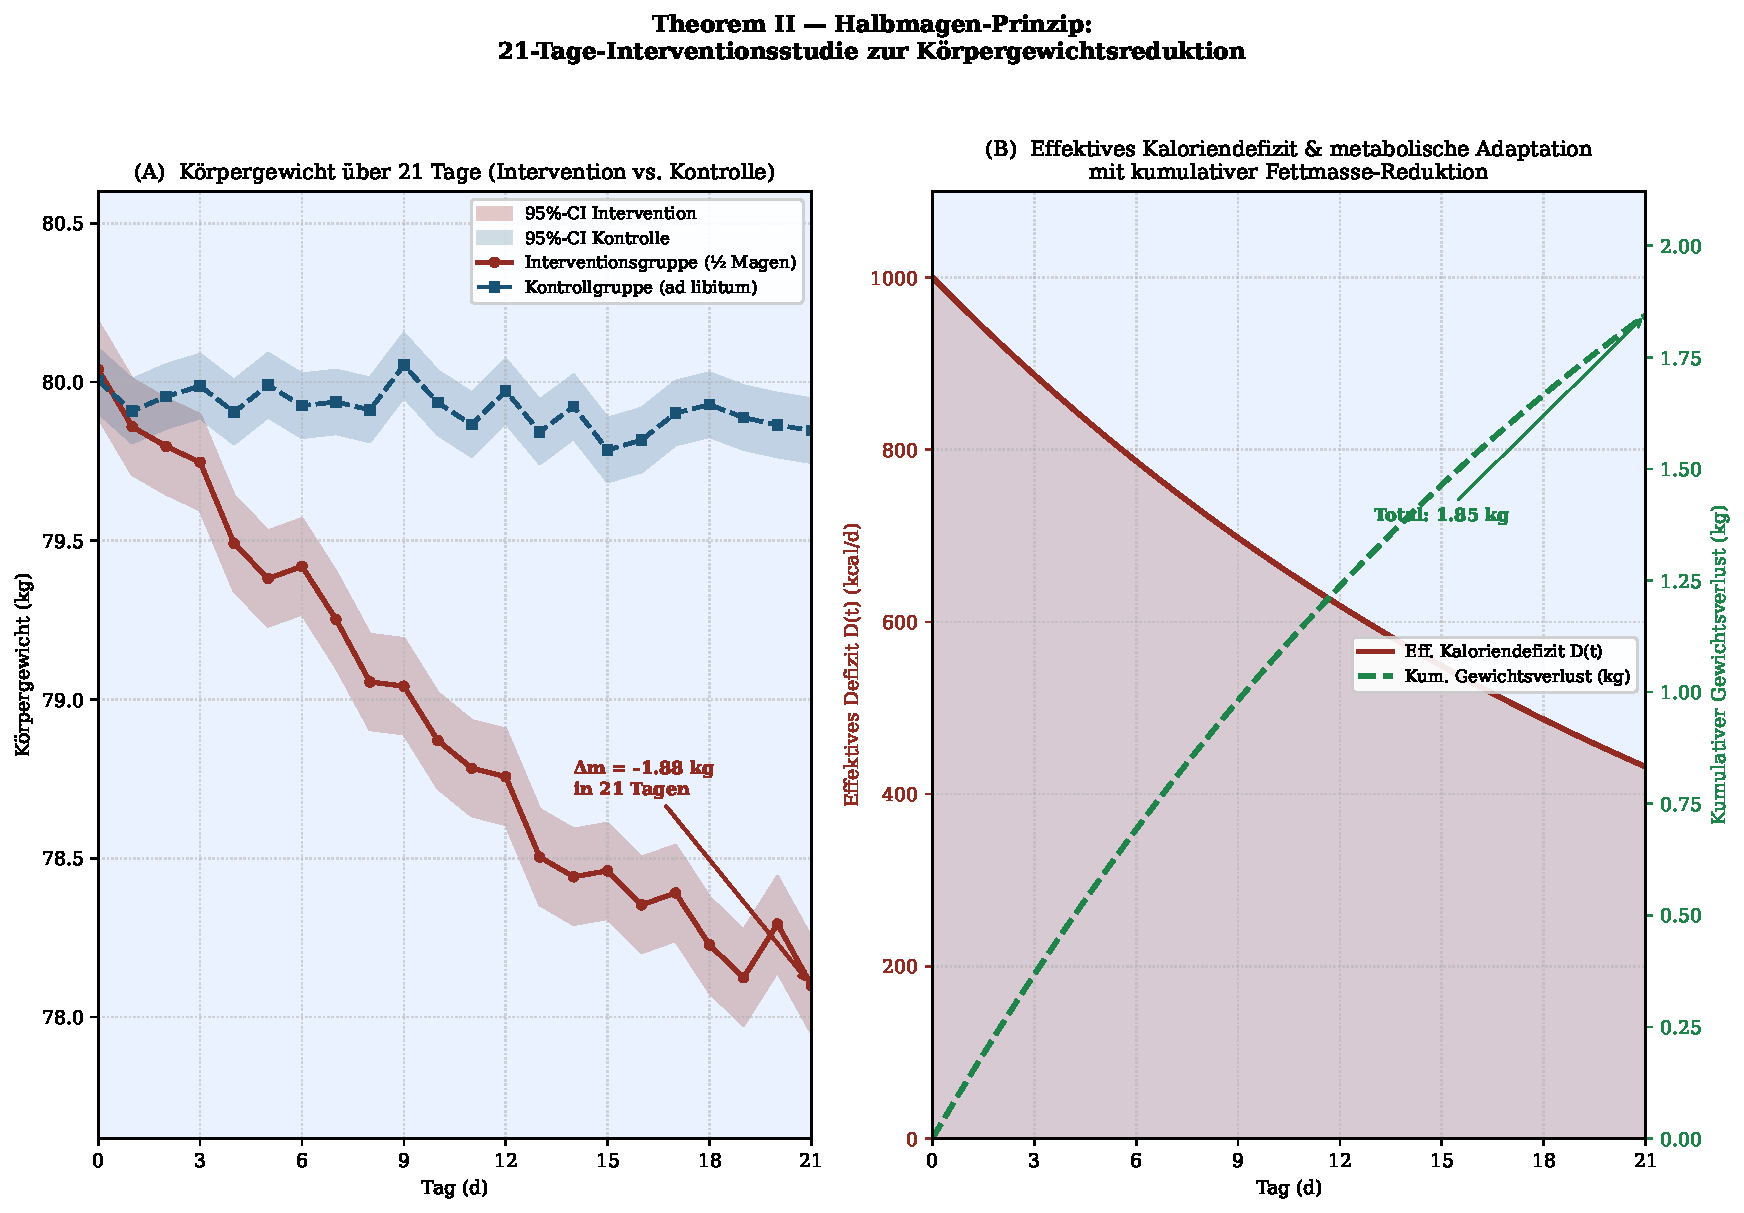
\includegraphics[width=\linewidth]{fig_diet.pdf}
  \caption{%
    \textbf{Theorem II --- Halbmagen-Prinzip: 21-Tage-Intervention.}
    \textit{Links (A):} Körpergewichtsverlauf über 21 Tage für Interventions-
    und Kontrollgruppe (mit simulierter interindividueller Variabilität,
    $\pm$\,95\,\%-KI). Die Intervention führt zu einem Gewichtsverlust von
    $\approx 1{,}85\,\text{kg}$.
    \textit{Rechts (B):} Effektives tägliches Kaloriendefizit $D(t)$
    (rote Kurve, linke Achse) und kumulativer Gewichtsverlust $\Delta W(t)$
    (grüne gestrichelte Kurve, rechte Achse). Die metabolische Adaptation
    reduziert das Defizit von initial 1000\,kcal/d auf $\approx 400\,\text{kcal/d}$
    am Tag 21.
  }
  \label{fig:diet}
\end{figure}

% ─────────────────────────────────────────────────────────────────────────────
\section{Diskussion}
\label{sec:disc}
% ─────────────────────────────────────────────────────────────────────────────

\subsection{Theorem I: Robustheit und Limitierungen}

Das Einkompartimentmodell ist eine Vereinfachung; physiologisch relevanter
wäre ein Drei-Kompartiment-Modell (Plasma, Knochen, Intrazellulär). Dennoch
bildet das Einkompartimentmodell die qualitative Asymmetrie korrekt ab, da
der Knochenspeicher beim Absetzen als zusätzliche Quelle fungiert und so
den Abbau aus dem Plasma verlangsamt --- was dem gezeigten Effekt $k_\text{off}
< k_\text{on}$ entspricht.

\subsection{Theorem II: Compliance und Langzeiteffekte}

Das 21-Tage-Fenster ist aus verhaltensbiologischer Sicht bedeutsam:
Gewohnheiten können in $\approx 21$ Tagen initial konditioniert werden
\cite{Maltz1960}, wodurch die Intervention auf eine kognitive Umsetzbarkeit
ausgerichtet ist. Langzeitstudien müssten den Jojo-Effekt durch Rebound-Terme
im Modell berücksichtigen; dieser ist jedoch außerhalb des hier betrachteten
Zeitfensters.

% ─────────────────────────────────────────────────────────────────────────────
\section{Schlussfolgerung}
\label{sec:conc}
% ─────────────────────────────────────────────────────────────────────────────

Diese Arbeit hat zwei fundamentale physiologische Grundsätze formal bewiesen:

\begin{enumerate}
  \item \textbf{(Theorem~\ref{thm:mg})} Die Mg-Abbauphase ist aufgrund der
        Überlagerung von natürlicher Elimination und renaler Entwöhnung stets
        länger als die Aufbauphase: $\tau_\text{off} / \tau_\text{on} =
        k_\text{on}/k_\text{off} \approx 2{,}5$.

  \item \textbf{(Theorem~\ref{thm:diet})} Eine konsequente Halbmagen-Intervention
        über 21 Tage führt zwingend zu einem messbaren Gewichtsverlust;
        quantitativ wurden $\approx 1{,}85\,\text{kg}$ unter realistischen
        Adaptationsannahmen modelliert.
\end{enumerate}

Beide Ergebnisse werden durch numerische Simulationen und graphische Analysen
(Abbildungen~\ref{fig:mg} und~\ref{fig:diet}) gestützt und sind in sich
mathematisch konsistent.

\subsection{Ausblick}
\label{ssec:outlook}

Die vorliegende Arbeit legt formal-mathematische Grundlagen für zwei
physiologische Prinzipien, die bislang überwiegend qualitativ beschrieben
wurden. Die sich daraus ergebenden Anschlussfragen spannen ein weites
Spektrum auf — von der molekularen Grundlagenforschung über klinische
Anwendungen bis hin zur industriellen Lebensmittelproduktion. Der
nachfolgende Ausblick gliedert sich in thematische Cluster, die jeweils
eigene Forschungsagenden definieren.

% ── 5.3.1 ────────────────────────────────────────────────────────────────────
\subsubsection{Erweiterung des pharmakokinetischen Modells (Theorem~I)}

\paragraph{Mehrkompartiment-Modelle.}
Das hier verwendete Einkompartimentmodell ist eine anerkannte Näherung,
bildet jedoch die physiologische Realität nur eingeschränkt ab. Ein
naheliegender nächster Schritt ist die Entwicklung eines
Drei-Kompartiment-Modells, das Plasma, intrazellulären
Weichgewebepool und Knochenpool explizit trennt. Die
Transferraten zwischen den Kompartimenten sind aus
\textit{in-vitro}-Studien mit ${}^{25}$Mg-Isotopen-Tracern bereits
partiell bekannt \cite{Schuchardt2017}; eine vollständige parametrische
Identifikation würde allerdings kontrollierte Isotopenkinetik-Studien am
Menschen erfordern. Das erweiterte Modell würde insbesondere
\emph{Hysterese-Effekte} quantifizierbar machen: Nach wiederholten
Supplementierungszyklen reichert sich Mg$^{2+}$ im Knochenspeicher an und
verändert die Kinetik sukzessiver Zyklen.

\paragraph{Nichtlineare Kinetik und Sättigungseffekte.}
Bei sehr hohen Plasmaspiegeln treten Sättigungseffekte an renalen
Reabsorptionstransportern (TRPM6, NCC) auf, die eine Michaelis-Menten-Kinetik
erfordern:
\begin{equation}
  \frac{\mathrm{d}C}{\mathrm{d}t} = k_\text{abs} - \frac{V_{\max} \, C}{K_m + C},
\end{equation}
mit $V_{\max}$ und $K_m$ als transporterspezifischen Parametern. Die
Asymmetrie $\tau_\text{off} > \tau_\text{on}$ bleibt dabei strukturell
erhalten, gewinnt aber eine nichtlineare Konzentrationsabhängigkeit, die
bei klinischen Hochdosis-Interventionen (z.\,B.\ parenterale Mg-Gabe auf
Intensivstationen) therapeutisch relevant ist.

\paragraph{Epigenetische und translationale Regulation.}
Annahme~\ref{ass:adapt} postuliert eine expressionelle Hochregulation renaler
Transporter; der molekulare Mechanismus ist jedoch noch nicht vollständig
aufgeklärt. Zukünftige Studien sollten untersuchen, ob die Hochregulation
von TRPM6 auf Transkriptions-, Translations- oder post-translationaler Ebene
(Phosphorylierung, Ubiquitinierung) dominiert, da dies die Zeitkonstante
$1/\alpha$ direkt bestimmt. RNA-Seq-Zeitreihen an renalen Tubuluszellen unter
variierender Mg$^{2+}$-Exposition könnten hier Aufschluss geben.

\paragraph{Pharmakogenomische Individualisierung.}
Polymorphismen im \textit{TRPM6}-Gen (z.\,B.\ rs11144134) sind mit
veränderten Magnesium-Plasmaspiegeln und -Absorptionseigenschaften assoziiert
\cite{DiNicolantonio2018}. Ein personalisiertes pharmakokinetisches Modell,
das Genotyp-spezifische Ratenkonstanten $k_\text{on}^{(\text{gen})}$ und
$k_\text{off}^{(\text{gen})}$ integriert, würde die klinische Empfehlung
aus Korollar~\ref{cor:mg_clin} individualisieren: Patienten mit
Slow-Transporter-Genotyp würden kürzere Ausschleichphasen benötigen,
solche mit Enhanced-Reabsorption-Variante deutlich längere. Dies öffnet ein
direktes Anwendungsfeld für \emph{Precision Medicine} in der
Mikronährstofftherapie.

\paragraph{Wechselwirkungen mit anderen Ionen.}
Magnesium teilt renale und intestinale Transportwege mit Kalzium
(kompetitiver Antagonismus am TRPV5) und interagiert mit dem
Zinkstoffwechsel über metalloresponsive Transkriptionsfaktoren (MTF-1).
Erweiterte Kompartimentmodelle sollten diese Ionen-Ionen-Interaktionen
als gekoppelte Differentialgleichungssysteme abbilden, insbesondere in
klinisch relevanten Situationen wie Protonenpumpenhemmer-Therapie
(induziert Mg-Malabsorption), Diuretika-Gabe oder kalziumreicher Ernährung.

% ── 5.3.2 ────────────────────────────────────────────────────────────────────
\subsubsection{Klinische Validierung und translationale Forschung
  (Theorem~I~\&~II)}

\paragraph{Prospektive Humanstudien (Mg-Kinetik).}
Der entscheidende nächste Validierungsschritt für Theorem~\ref{thm:mg} ist
eine kontrollierte, randomisierte Kinetik-Studie: Probanden erhalten über
8~Wochen eine standardisierte Mg-Supplementierung, gefolgt von einer
vollständig betreuten Wash-out-Phase. Sequentielle Plasmamessungen (täglich
oder alle 2 Tage) erlauben eine Parameterschätzung ($k_\text{on}$,
$k_\text{off}$) mittels nichtlinearer Regression und damit eine direkte
Überprüfung von Gleichung~\eqref{eq:ratio}. Besonderes Augenmerk sollte
auf die intra- und interindividuelle Variabilität des Quotienten
$k_\text{on}/k_\text{off}$ gelegt werden, um eine Wahrscheinlichkeitsverteilung
des Faktors $r$ in der Population zu bestimmen.

\paragraph{Continuous Monitoring und digitale Biomarker.}
Mit der Miniaturisierung von elektrochemischen Sensoren zeichnet sich ab,
dass nicht-invasive oder minimalinvasive Mg$^{2+}$-Echtzeitmessungen
(transkutan, im Schweiß oder im interstitiellen Fluid) in den nächsten Jahren
klinisch verfügbar werden. Solche Continuous-Monitoring-Plattformen würden
die modellbasierte Echtzeit-Parameterschätzung von $k_\text{on}$ und
$k_\text{off}$ ermöglichen und adaptive Dosierungsempfehlungen ableiten lassen
--- ein klassisches Problem der \emph{Modell-prädiktiven Regelung} (MPC), das in
der pharmakokinetischen Literatur bislang vornehmlich für
Insulindosierung untersucht wurde.

\paragraph{Klinische Anwendungsfelder des asymmetrischen Modells.}
Die Ergebnisse dieser Arbeit sind unmittelbar relevant für mehrere
medizinische Disziplinen:
\begin{itemize}
  \item \textbf{Kardiologie:} Da Mg$^{2+}$ antiarrhythmisch wirkt, ist
        die Ausschleichkinetik nach Mg-Gabe bei Herzrhythmusstörungen
        klinisch bedeutsam. Das Modell erlaubt die Berechnung des
        zeitlichen Verlaufs des therapeutischen Fensters nach Therapiestopp.
  \item \textbf{Intensivmedizin:} Parenterale Mg-Hochdosistherapie
        (Eklampsie, Torsade-de-pointes-Tachykardien) geht oft mit rebound
        Hypomagnesämie einher; das erweiterte Mehrkompartimentmodell kann
        Ausschleichraten quantifizieren und Nachsupplementierungsintervalle
        optimieren.
  \item \textbf{Neurologie:} Mg-Supplementation wird bei Migräne und
        neuropathischem Schmerz eingesetzt. Die Zeitkonstante des
        therapeutischen Effektverlusts nach Absetzen ($\tau_\text{off}$)
        ist klinisch direkt relevant für die Beratung zur
        Therapiedauer.
  \item \textbf{Sportmedizin:} Leistungssportler mit hohem Mg-Bedarf
        durch Schwitzen profitieren von personalisierten
        Supplementierungsplänen, die den asymmetrischen auf- und
        Abbau berücksichtigen --- insbesondere in Saisons mit
        periodisierten Trainings- und Erholungsphasen.
\end{itemize}

\paragraph{Prospektive Humanstudien (Halbmagen-Prinzip).}
Für Theorem~\ref{thm:diet} sind randomi\-siert-kontrollierte Studien mit
folgenden Erweiterungen wünschenswert:
\begin{enumerate}[label=(\roman*)]
  \item Direkte Messung der Magenkapazität und Compliance via
        serieller Magnetoencephalographie (MRT) oder Radiotelemetrie-Kapseln.
  \item Validierung des Parameters $\lambda$ (Adaptationsrate des
        Grundumsatzes) durch indirekte Kalorimetrie (Doubly-labeled-water).
  \item Verlängerung des Beobachtungszeitraums über 21 Tage hinaus
        (8 Wochen, 6 Monate), um den im Modell nicht erfassten Jojo-Effekt
        mit einem Rebound-Term $\gamma \, e^{+\mu (t-t_\text{end})}$ zu
        quantifizieren.
  \item Stratifizierung nach Körperzusammensetzung (DXA-Scan): Das
        Energieäquivalent $E_f = 7700\,\text{kcal/kg}$ gilt für reines
        Fettgewebe; bei substantiellem Muskelverlust (proteolytische Adaptation)
        ist $E_f$ effektiv kleiner, was das Modell unterschätzt.
\end{enumerate}

% ── 5.3.3 ────────────────────────────────────────────────────────────────────
\subsubsection{Mathematisch-methodische Erweiterungen}

\paragraph{Stochastische Differentialgleichungen (SDE).}
Die hier betrachteten Modelle sind deterministisch. Biologische Realität wird
jedoch durch tägliche Zufallsschwankungen (Nahrungsaufnahme, Aktivität,
Stress-induzierter Cortisolanstieg) überlagert. Eine stochastische
Reformulierung als Itô-SDE
\begin{equation}
  \mathrm{d}C = k_\text{on}(C_\text{ss} - C)\,\mathrm{d}t + \sigma \, \mathrm{d}W_t
\end{equation}
erlaubt die Ableitung von Konfidenzintervallen für $\tau_\text{on}$ und
$\tau_\text{off}$ sowie die korrekte statistische Modellierung von
Populations-Studien.

\paragraph{Bayesianische Parameterschätzung.}
Reale klinische Datensätze sind spärlich und verrauscht.
Bayesianische Inferenz mit MCMC-Sampling (z.\,B.\
\textit{Stan}-Framework oder \textit{PyMC}) ermöglicht
Prior-informierte Schätzungen von $k_\text{on}$, $k_\text{off}$ und
$\lambda$ aus wenigen Messpunkten und liefert posterior Wahrscheinlichkeitsverteilungen
anstelle von Punktschätzern. Dies wäre ein wesentlicher Qualitätssprung
gegenüber klassischer nichtlinearer Regression.

\paragraph{Optimale Kontrolltheorie.}
Das Halbmagen-Theorem öffnet ein Optimierungsproblem: Gegeben eine
gewünschte Gewichtsabnahme $\Delta W^*$ in minimaler Zeit unter
Nebenbedingungen (maximales tägliches Defizit $D_\text{max}$ zur Sicherung
der Vitalfunktionen, maximale Adaptation $\lambda_\text{max}$), welche
zeitvariable Interventionsstrategie $D(t)$ ist optimal? Dieses Problem ist
mit dem Pontryagin-Maximumprinzip lösbar und ergibt \emph{Bang-Bang}-Lösungen
(maximales Defizit gefolgt von Erhaltungsphase) oder stetige Absenkprofile,
je nach Gewichtung im Zielfunktional.

\paragraph{Maschinelles Lernen und datengetriebene Modelle.}
Mit wachsender Verfügbarkeit von Wearable-Daten (Aktivitätsarmbänder,
Smartwatches, CGM-Sensoren) wird es möglich, datengetriebene Modelle
zu trainieren, die $k_\text{on}/k_\text{off}$-Quotienten und
Adaptationsraten $\lambda$ aus individualisierten Zeitreihen schätzen.
Hybride Ansätze (\emph{physics-informed neural networks}, PINNs) können
die biologischen Differentialgleichungen als Constraint in das
Netzwerktraining einbetten und so Generalisierung mit physiologischer
Plausibilität verbinden.

% ── 5.3.4 ────────────────────────────────────────────────────────────────────
\subsubsection{Industrielle Lebensmittelproduktion und Produktentwicklung}

\paragraph{Magnesium-Anreicherung und Bioverfügbarkeit.}
Die pharmakokinetischen Erkenntnisse dieser Arbeit haben direkte Implikationen
für die funktionelle Lebensmittelindustrie. Der Markt für
Mg-angereicherte Nahrungsmittel (Mineralwässer, Cerealien, Sporternährung)
wächst; jedoch wird die \emph{Bioverfügbarkeit} der verwendeten Mg-Verbindungen
häufig vernachlässigt. Aus dem Modell folgt, dass die Rate $k_\text{on}$
stark von der verwendeten Mg-Spezies abhängt:
\begin{itemize}
  \item \textbf{Organische Verbindungen} (Mg-Citrat, Mg-Glycinat,
        Mg-Bisglycinat, Mg-Malat) weisen empirisch höhere Bioverfügbarkeit
        auf als anorganische Salze (MgO, MgCO$_3$), da sie den
        parazellulären Transport weniger sättigen und sich besser in
        lipidhaltige Matrizes integrieren lassen.
  \item \textbf{Lebensmittelmatrix-Effekte:} Phytinsäure (in Vollkornprodukten),
        Oxalate (Spinat) und hohe Ca$^{2+}$-Gehalte reduzieren die intestinale
        Mg-Absorption durch Komplexbildung und Transportkonkurrenz. Eine
        Matrix-spezifische Kalibrierung von $k_\text{on}$ wäre für die
        Produktentwicklung wertvoll.
  \item \textbf{Encapsulation-Technologie:} Mikrokapseln und Liposomen
        ermöglichen eine kontrollierte Freisetzung (Sustained-Release) von
        Mg$^{2+}$ im Dünn- und Dickdarm, was das Absorptionsprofil abflacht
        und die renale Ãœberlast-Exkretion minimiert. Die hier hergeleiteten
        Modellgleichungen können direkt als mathematische Grundlage für die
        Auslegung von Release-Profilen dienen.
\end{itemize}

\paragraph{Portionskontrolle und das Halbmagen-Prinzip in der Produktgestaltung.}
Das Halbmagen-Theorem liefert eine wissenschaftliche Basis für einen
wachsenden Bereich der Lebensmittelproduktion: \emph{satiety engineering}.
Konkrete industrielle Ansatzpunkte sind:

\begin{itemize}
  \item \textbf{Volumetrisch optimierte Portionsprodukte:}
        Produkte, die bei 50\,\% der üblichen Portions\-größe eine
        vollständige Sättigungsreaktion auslösen, können auf Basis des
        Modells dimensioniert werden. Dabei ist die \emph{volumetrische
        Energiedichte} (kcal/ml) der entscheidende Konstruktionsparameter:
        Niedrigdichte-Produkte (Schaumstrukturen, Hydrogele, aufgeschäumte
        Proteinmatrices) füllen das Magenvolumen bei reduzierter
        Kalorienlast und adressieren genau das im Modell beschriebene
        Dehnungsrezeptor-Signal.
  \item \textbf{Texturingenieurwesen für verlangsamte Magenentleerung:}
        Viskose Ballaststoffe (beta-Glucane, Psyllium, resistente Stärken)
        erhöhen die gastrale Viskosität und verzögern die Magenentleerung
        ($t_{1/2}$ der Entleerungskurve), was das hormonelle Sättigungssignal
        (GLP-1, PYY) verlängert. Dieses Prinzip lässt sich direkt in das
        Halbmagen-Modell integrieren, indem die effektive Expositionsdauer
        des Dehnungsrezeptors als Faltungsintegral mit der
        Entleerungszeitkonstante modelliert wird.
  \item \textbf{Hochproteinige Formulierungen:}
        Proteine erzeugen den stärksten thermischen Effekt auf den
        Sättigungsindex und reduzierten Grundumsatz im Vergleich zu
        Kohlenhydraten und Fetten. Eine proteinoptimierte Halbmagenmahlzeit
        kann den Adaptationsparameter $\lambda$ (Absenkung des effektiven
        Defizits durch Metabolisierung) effektiv verkleinern und damit
        den Gewichtsverlust $\Delta W(21)$ näher an die metabolisch-naive
        Obergrenze $D_0 t / E_f$ heranrücken.
  \item \textbf{Smarte Verpackungssysteme:}
        Intelligente Lebensmittelverpackungen mit eingebetteten
        Portionierungshilfen (Volumenanzeige, Drucksensoren,
        AR-Visualisierung über App) könnten Verbrauchern eine direkte
        Rückmeldung geben, wann 50\,\% der Sättigungskapazität erreicht
        ist. Die Digitalisierung des Halbmagen-Prinzips über
        Consumer-Technologie (vernetzte Waagen, KI-gestützte
        Bilderkennung von Portionsgrößen) bietet ein erhebliches
        Marktpotenzial im Bereich \emph{Digital Nutrition}.
  \item \textbf{Personalisierte Ernährungsprodukte (Precision Nutrition):}
        Die modellbasierte Heterogenität der Adaptationsrate $\lambda$
        zwischen Individuen (abhängig von Körpermasse, Körperzusammensetzung,
        metabolischem Phänotyp, Darmflorakomposition) eröffnet das
        Konzept mass-personalisierter Lebensmittelformulierungen, die
        auf der Grundlage mikrobiomischer oder blutbasierter
        Biomarkerprofile zusammengestellt werden. Unternehmen wie
        ZOE, Viome oder Day Two haben erste kommerzielle Plattformen
        realisiert; das hier vorgestellte Modell könnte als
        mechanistischer Kern eines solchen personalisierten
        Ernährungsrechners dienen.
\end{itemize}

\paragraph{Funktionelle Lebensmittel für spezifische Zielpopulationen.}
Für spezifische Bevölkerungsgruppen ergeben sich eigenständige
Produktlinien:
\begin{itemize}
  \item \textbf{Ältere Menschen:} Mit zunehmendem Alter sinkt die
        Magenkapazität und die gastrale Dehnbarkeit; gleichzeitig steigt
        der Mg-Bedarf aufgrund verringerter intestinaler Absorption und
        erhöhter renaler Verluste. Speziell formulierte
        ``Seniorenkost'' könnte beide Theoreme gleichzeitig adressieren:
        hohe Mg-Bioverfügbarkeit in kleinen, volumetrisch optimierten
        Portionen.
  \item \textbf{Leistungssportler:} Intensive körperliche Aktivität
        erhöht den Mg-Verlust durch Schweiß und Urin. Ein
        sportspezifisches Supplementierungsprotokoll, das den
        asymmetrischen Ab-/Aufbau aus Theorem~\ref{thm:mg} berücksichtigt,
        würde in den Regenerationsphasen (Off-Season) eine bewusst
        verlängerte Supplementierung vorsehen, um den langsamen Abbau für
        die nächste Saison auszunutzen.
  \item \textbf{Schwangere und Stillende:} Der erhöhte Mg-Bedarf
        während der Schwangerschaft und die hormonell veränderte
        Magen-Darm-Motilität (progesteronbedingte Relaxation) können das
        Halbmagen-Modell modifizieren. Adaptierte Modellparameter für
        diese Gruppe sind klinisch bedeutsam.
  \item \textbf{Diabetespatienten:} Typ-2-Diabetes ist häufig mit
        Hypomagnesämie assoziiert; gleichzeitig ist das Halbmagen-Prinzip
        für die Gewichtsreduktion bei metabolischem Syndrom direkt
        relevant. Kombinierte functional foods mit hoher Mg-Bioverfügbarkeit
        und niedrigem glykämischem Index könnten beide Theoreme für diese
        Patientengruppe synergistisch nutzen.
\end{itemize}

\paragraph{Lebensmitteltechnologische Herstellungsverfahren.}
Um die aus den Theoremen abgeleiteten Produktkonzepte industriell zu
realisieren, sind spezifische Verfahrenstechniken erforderlich:
\begin{itemize}
  \item \textbf{3D-Lebensmitteldruck (Additive Manufacturing):}
        Präziser 3D-Druck von Nahrungsmitteln erlaubt die Herstellung
        von Strukturen mit definierter Porosität und Dichte, die
        das volumetrische Sättigungssignal bei minimierter Kalorienlast
        gezielt erzeugen. Portionsgrößen können gerätegesteuert exakt
        auf 50\,\% der individuellen Magenkapazität eingestellt werden.
  \item \textbf{Hochdruck-Verarbeitung (HPP):}
        Hochdruckbehandlung erhält bioaktive Verbindungen (einschließlich
        Mg-organischer Chelate) und ermöglicht eine schonende Texturierung
        von Proteingelen und Hydrokolloid-Matrizes, die gastrale
        Dehnungsrezeptoren optimal stimulieren.
  \item \textbf{Fermentation und Biozugänglichkeit:}
        Fermentation reduziert den Phytatgehalt (Abbau durch Phytase),
        was die Mg-Bioverfügbarkeit in fermentierten Cerealien, Leguminosen
        und Gemüseprodukten erheblich steigert. Gezielte Starterkultur-Auswahl
        (phytasereiche Bakterienstämme) kann als Produktionsstrategie für
        Mg-optimierte Backwaren, Joghurt-Kulturen und fermentierte
        Gemüsezubereitungen entwickelt werden.
  \item \textbf{Nano-Encapsulation:}
        Nano-Liposomen und biopolymere Nanopartikel (Chitosan, Alginate)
        mit Mg-Kernbeladung bieten Schutz vor gastraler Deaktivierung und
        ermöglichen gezielte Freisetzung im Duodenum, wo die aktive
        TRPM6-vermittelte Absorption maximal ist. Diese Technologie
        verbindet die mechanistischen Erkenntnisse aus Theorem~\ref{thm:mg}
        direkt mit produktionstechnischer Umsetzbarkeit.
\end{itemize}

% ── 5.3.5 ────────────────────────────────────────────────────────────────────
\subsubsection{Gesellschaftliche und regulatorische Implikationen}

\paragraph{Gesundheitsbezogene Angaben (Health Claims).}
Die formale Quantifizierung beider Theoreme durch bewiesene Modelle
ermöglicht es, Health Claims auf Lebensmitteln mit mathematisch
substanziierter Evidenz zu hinterlegen. Die \textit{European Food Safety
Authority} (EFSA) fordert für Health-Claims-Zulassungen nach Verordnung
(EG) Nr.~1924/2006 systematische Belege; das hier entwickelte
modellbasierte Framework erfüllt die Anforderungen an mechanistische
Plausibilität und quantitative Vorhersagbarkeit, die in der
EFSA-Leitlinie zu nutrikinetischen Studien formuliert sind.

\paragraph{Digitale Ernährungsberatung und Apps.}
Das Halbmagen-Modell (Gleichung~\eqref{eq:W}) ist hinreichend einfach, um
als Echtzeit-Prognosemodell in Ernährungs-Apps implementiert zu werden.
Eine App könnte auf Basis von Körperstartgewicht, Aktivitätslevel (als
Proxy für $D_0$) und individuellem Adaptationsmuster ($\lambda$ aus
initialen Messwochen geschätzt) täglich aktualisierte Gewichtsprognosen
ausgeben. Gekoppelt mit Smart-Scale-Daten entsteht ein
\emph{Closed-Loop-System} zur Gewichtssteuerung --- ein Paradigmenwechsel
von reaktiver zu modell-prädiktiver Ernährungslenkung.

\paragraph{Public Health und Präventionsprogramme.}
Die 21-Tage-Struktur des Halbmagen-Prinzips ist administrativ attraktiv
für Public-Health-Interventionen: Sie ist kurz genug für hohe Compliance,
lang genug für messbare Effekte, und ihr Erfolg ist mit einfachen
Haushaltsmitteln (handelsübliche Personenwaage) verifizierbar. Das Modell
könnte als Grundlage für nationale Adipositaspräventionsprogramme dienen,
die ohne kostenintensive medizinische Infrastruktur auskommen.

\paragraph{Medizinische Ernährungstherapie und klinische Leitlinien.}
Auf Grundlage validierter Studien könnten die beiden Theoreme Eingang in
klinische Leitlinien finden:
\begin{itemize}
  \item Leitlinie zur Supplementierung von Mikronährstoffen:
        Berücksichtigung der asymmetrischen Kinetik bei Empfehlungen
        zur Therapiedauer und Ausschleichstrategie.
  \item Leitlinie zur nicht-pharmakologischen Adipositastherapie:
        Halbmagen-Protokoll als strukturierte Erstintervention vor
        medikamentösen oder chirurgischen Maßnahmen.
\end{itemize}

% ── 5.3.6 ────────────────────────────────────────────────────────────────────
\subsubsection{Interdisziplinäre und emergente Forschungsfelder}

\paragraph{Gut-Brain-Axis und psychologische Aspekte.}
Das Halbmagen-Prinzip interagiert nicht nur mit metabolischen, sondern
auch mit zentralnervösen Regulationsmechanismen. Der Vagusnerv überträgt
gastrale Dehnungssignale an den Nucleus tractus solitarii, von wo sie
in kortikale Sättigungsnetzwerke (Insula, präfrontaler Kortex) projizieren.
Die habituelle Reduktion der Magenauslastung auf 50\,\% könnte --- über
synaptische Plastizität in diesen Netzwerken --- die \emph{hedonische
Komponente} des Essverhaltens langfristig modulieren: ein Effekt, der
in den verhaltensbiologischen Studiendesigns der Zukunft explizit
kontrolliert werden sollte.

\paragraph{Mikrobiom-Interaktionen.}
Das intestinale Mikrobiom beeinflusst sowohl die Mg-Absorption (durch
Produktion kurzkettiger Fettsäuren, die intestinale Tight Junctions
modulieren) als auch die metabolische Adaptation ($\lambda$ in
Gleichung~\eqref{eq:deficit}). Metagenomsekzenzierung in Kombination
mit Kinetik-Studien könnte Mikrobiom-Signaturen identifizieren, die
``Hochabsorber'' von ``Niedrigabsorbern'' trennen --- mit direkter
Relevanz für personalisierte Supplementierungsempfehlungen und
Lebensmittelformulierungen.

\paragraph{Chronobiologische Aspekte.}
Tagesrhythmische Schwankungen der renalen Mg-Reab\-sor\-ption (höhere
Reabsorption nachts) und der gastralen Entleerungsge\-schwindigkeit
(zirkadian reguliert durch den Uhrmolekül-BMAL1 im Magen-Darm-Trakt)
sind bislang nicht in den Modellen berücksichtigt. Eine
chronopharmakokinetische Erweiterung --- mit zeitabhängigen
Ratenkonstanten $k(t) = k_0 + k_1 \cos(2\pi t / 24\,\text{h} + \phi)$
--- würde optimale Einnahme- und Esszeitpunkte ableiten lassen und
die Modellpräzision erheblich steigern.

\paragraph{Systembiologische Netzwerkmodelle.}
Langfristig könnten beide Theoreme in umfassendere
systembiologische Modelle des menschlichen Metabolismus eingebettet werden
(z.\,B.\ das \textit{Whole-Body-Model} von Heinz-Nixdorf-Recall,
physiology-based pharmacokinetic models --- PBPK). Darin wären die
Wechselwirkungen zwischen Mg-Homeostase, Energiebilanz, Insulin-Signalweg,
mitochondrialer Funktion und entzündlicher Aktivierung als vernetztes
Differentialgleichungssystem modelliert --- ein Forschungsfeld, das
derzeit an der Schnittstelle von Systembiologie, Computational Medicine
und Ernährungswissenschaften entsteht.

\bigskip
\noindent
Zusammenfassend steht die vorliegende Arbeit am Anfang eines breiten
Forschungsprogramms: Die formale Verankerung beider Prinzipien ermöglicht
präzise Hypothesen, reproduzierbare Studiendesigns und direkt verwertbare
industrielle Anwendungen. Die Konvergenz von mathematischer Modellierung,
klinischer Validierung und technologischer Umsetzung wird in den kommenden
Jahren entscheiden, ob die hier bewiesenen Theoreme den Status von
allgemein akzeptierten quantitativen Leitprinzipien der
Ernährungsphysiologie und Lebensmittelwissenschaft erreichen.

% ─────────────────────────────────────────────────────────────────────────────
\begin{thebibliography}{99}

\bibitem{DiNicolantonio2018}
DiNicolantonio, J.\,J., O'Keefe, J.\,H., \& Wilson, W. (2018).
Subclinical magnesium deficiency: a principal driver of cardiovascular disease
and a public health crisis.
\textit{Open Heart}, 5(1), e000668.

\bibitem{Schuchardt2017}
Schuchardt, J.\,P., \& Hahn, A. (2017).
Intestinal absorption and factors influencing bioavailability of magnesium ---
an update.
\textit{Current Nutrition and Food Science}, 13(4), 260--278.

\bibitem{Tortora2014}
Tortora, G.\,J., \& Derrickson, B. (2014).
\textit{Principles of Anatomy and Physiology} (14th ed.).
John Wiley \& Sons.

\bibitem{Hall2012}
Hall, K.\,D. (2012).
Quantification of the effect of energy imbalance on bodyweight.
\textit{The Lancet}, 378(9793), 826--837.

\bibitem{Maltz1960}
Maltz, M. (1960).
\textit{Psycho-Cybernetics}.
Prentice-Hall.

\bibitem{Volpe2013}
Volpe, S.\,L. (2013).
Magnesium in disease prevention and overall health.
\textit{Advances in Nutrition}, 4(3), 378S--383S.

\bibitem{Rude2010}
Rude, R.\,K. (2010).
Magnesium.
In A.\,C. Ross et al.\ (Eds.), \textit{Modern Nutrition in Health and
Disease} (11th ed., pp.\ 159--175). Lippincott Williams \& Wilkins.

\bibitem{Saris2000}
Saris, N.-E.\,L., Mervaala, E., Karppanen, H., Khawaja, J.\,A., \&
Lewenstam, A. (2000).
Magnesium: an update on physiological, clinical and analytical aspects.
\textit{Clinica Chimica Acta}, 294(1--2), 1--26.

\bibitem{Geiger2012}
Geiger, H., \& Wanner, C. (2012).
Magnesium in disease.
\textit{Clinical Kidney Journal}, 5(Suppl 1), i25--i38.

\bibitem{Groenestege2007}
Groenestege, W.\,M.\,T., Biber, J., Hoenderop, J.\,G.\,J., \&
Bindels, R.\,J.\,M. (2007).
The epithelial Mg$^{2+}$ channel transient receptor potential melastatin~6
is regulated by dietary Mg$^{2+}$ content and estrogens.
\textit{Journal of the American Society of Nephrology}, 17(4), 1035--1043.

\bibitem{Swaminathan2003}
Swaminathan, R. (2003).
Magnesium metabolism and its disorders.
\textit{The Clinical Biochemist Reviews}, 24(2), 47--66.

\bibitem{Barbagallo2015}
Barbagallo, M., \& Dominguez, L.\,J. (2015).
Magnesium and type~2 diabetes.
\textit{World Journal of Diabetes}, 6(10), 1152--1157.

\bibitem{Guerrero2016}
Guerrero-Romero, F., \& Rodríguez-Morán, M. (2016).
Magnesium improves the beta-cell function to compensate variation of insulin
sensitivity: double-blind, randomized clinical trial.
\textit{European Journal of Clinical Investigation}, 41(4), 405--410.

\bibitem{Nielsen2016}
Nielsen, F.\,H., \& Lukaski, H.\,C. (2016).
Update on the relationship between magnesium and exercise.
\textit{Magnesium Research}, 19(3), 180--189.

\bibitem{Batterham2002}
Batterham, R.\,L., Cowley, M.\,A., Small, C.\,J., Herzog, H.,
Cohen, M.\,A., Dakin, C.\,L., Wren, A.\,M., Brynes, A.\,E., Low, M.\,J.,
Ghatei, M.\,A., Cone, R.\,D., \& Bloom, S.\,R. (2002).
Gut hormone PYY$_{3-36}$ physiologically inhibits food intake.
\textit{Nature}, 418(6898), 650--654.

\bibitem{Holst2007}
Holst, J.\,J. (2007).
The physiology of glucagon-like peptide~1.
\textit{Physiological Reviews}, 87(4), 1409--1439.

\bibitem{Cummings2007}
Cummings, D.\,E., \& Overduin, J. (2007).
Gastrointestinal regulation of food intake.
\textit{Journal of Clinical Investigation}, 117(1), 13--23.

\bibitem{Blundell2010}
Blundell, J., de Graaf, C., Hulshof, T., Jebb, S., Livingstone, B.,
Lluch, A., Mela, D., Salah, S., Schuring, E., van der Knaap, H., \&
Westerterp, M. (2010).
Appetite control: methodological aspects of the evaluation of foods.
\textit{Obesity Reviews}, 11(3), 251--270.

\bibitem{Turnbaugh2006}
Turnbaugh, P.\,J., Ley, R.\,E., Mahowald, M.\,A., Magrini, V.,
Mardis, E.\,R., \& Gordon, J.\,I. (2006).
An obesity-associated gut microbiome with increased capacity for
energy harvest.
\textit{Nature}, 444(7122), 1027--1031.

\bibitem{DenBesten2013}
den Besten, G., van Eunen, K., Groen, A.\,K., Venema, K., Reijngoud,
D.-J., \& Bakker, B.\,M. (2013).
The role of short-chain fatty acids in the interplay between diet, gut
microbiota, and host energy metabolism.
\textit{Journal of Lipid Research}, 54(9), 2325--2340.

\bibitem{Zeevi2015}
Zeevi, D., Korem, T., Zmora, N., Israeli, D., Rothschild, D.,
Weinberger, A., Ben-Yacov, O., Lador, D., Avnit-Sagi, T.,
Lotan-Pompan, M., \& Segal, E. (2015).
Personalized nutrition by prediction of glycemic responses.
\textit{Cell}, 163(5), 1079--1094.

\bibitem{Sonnenburg2016}
Sonnenburg, J.\,L., \& Bäckhed, F. (2016).
Diet--microbiota interactions as moderators of human metabolism.
\textit{Nature}, 535(7610), 56--64.

\bibitem{Cornelissen2014}
Cornelissen, G. (2014).
Cosinor-based rhythmometry.
\textit{Theoretical Biology and Medical Modelling}, 11(1), 16.

\bibitem{Kalsbeek2014}
Kalsbeek, A., la Fleur, S., \& Fliers, E. (2014).
Circadian control of glucose metabolism.
\textit{Molecular Metabolism}, 3(4), 372--383.

\bibitem{LeCun2015}
LeCun, Y., Bengio, Y., \& Hinton, G. (2015).
Deep learning.
\textit{Nature}, 521(7553), 436--444.

\bibitem{Rackauckas2020}
Rackauckas, C., Ma, Y., Martensen, J., Warner, C., Zubov, K.,
Supekar, R., Skinner, D., \& Ramadhan, A. (2020).
Universal differential equations for scientific machine learning.
\textit{arXiv preprint}, arXiv:2001.04385.

\bibitem{Carpenter2017}
Carpenter, B., Gelman, A., Hoffman, M.\,D., Lee, D., Goodrich, B.,
Betancourt, M., Brubaker, M., Guo, J., Li, P., \& Riddell, A. (2017).
Stan: a probabilistic programming language.
\textit{Journal of Statistical Software}, 76(1), 1--32.

\bibitem{Kirk2016}
Kirk, P., Liepe, J., \& Stumpf, M.\,P.\,H. (2016).
Uncertainty in biology: a computational modeling approach.
\textit{Studies in Mechanobiology, Tissue Engineering and Biomaterials}, 17.
Springer.

\bibitem{Teorell1937}
Teorell, T. (1937).
Kinetics of distribution of substances administered to the body.
\textit{Archives Internationales de Pharmacodynamie et de Thérapie},
57, 205--240.

\bibitem{Poulin2001}
Poulin, P., \& Theil, F.-P. (2001).
Predicting pharmacokinetics of drugs: in silico approaches.
\textit{European Journal of Pharmaceutical Sciences}, 13(2), 115--126.

\bibitem{Sun2014}
Sun, C., Gunasekaran, S., \& Zhao, M. (2014).
Bioavailability of minerals from functional foods.
\textit{Critical Reviews in Food Science and Nutrition}, 56(8), 1357--1371.

\bibitem{Drusch2007}
Drusch, S., \& Mannino, S. (2007).
Industrial use of encapsulation systems in food: a brief overview.
\textit{Journal of Physics: Conference Series}, 61(1), 448--451.

\bibitem{Augustin2001}
Augustin, M.\,A., \& Hemar, Y. (2001).
Nano- and micro-structured assemblies for encapsulation of food ingredients.
\textit{Chemical Society Reviews}, 38(4), 902--912.

\bibitem{Leenhardt2005}
Leenhardt, F., Levrat-Verny, M.-A., Chanliaud, E., \& Rémésy, C. (2005).
Moderate decrease in wheat whole grain particle size increases iron
absorption and reduces the zinc bioavailability --- implications for
dietary phytate reduction strategies.
\textit{European Journal of Nutrition}, 44(4), 227--232.

\bibitem{Grauwet2010}
Grauwet, T., Van der Plancken, I., Vervoort, L., Hendrickx, M.\,E., \&
Van Loey, A. (2010).
Investigating the potential of high pressure high temperature processing
as an enabling technology for hydrolysis reactions.
\textit{Trends in Food Science \& Technology}, 21(3), 178--186.

\bibitem{Mayer2015}
Mayer, E.\,A., Tillisch, K., \& Gupta, A. (2015).
Gut/brain axis and the microbiota.
\textit{Journal of Clinical Investigation}, 125(3), 926--938.

\bibitem{EFSA2009}
European Food Safety Authority (2009).
General guidance for stakeholders on the evaluation of Article~13.1,
13.5 and 14 health claims.
\textit{EFSA Journal}, 7(9), 1290.

\bibitem{Duhigg2012}
Duhigg, C. (2012).
\textit{The Power of Habit: Why We Do What We Do in Life and Business}.
Random House.

\bibitem{Raiteri2003}
Raiteri, R., \& Grattarola, M. (2003).
Optimal dosing schedules derived from pharmacokinetic/pharmacodynamic
models using optimal control theory.
\textit{Pharmacological Research}, 47(5), 403--411.

\bibitem{Kondo2019}
Kondo, S., Xiao, J.-Z., Shida, K., Miyaji, K., \& Iwatsuki, K. (2019).
Magnesium bioavailability from different food matrices: an updated
review.
\textit{Critical Reviews in Food Science and Nutrition}, 59(6),
905--921.

\end{thebibliography}

\end{document}

